% !Mode:: "TeX:UTF-8"

\chapter[模拟退火算法]{模拟退火算法}
\section{模拟退火算法介绍}
  模拟退火算法(Simmulated Annealing Method),简称SA,由Kirpatrick et al\cite{obsa}
在Metropolis et al的基础工作之上提出,Metropolis当时已经实现了单机和并行的算法,能够解决
大部分非常困难的组合优化问题.模拟退火算法基于统计力学和组合优化的类比问题.

 模拟退火算法来源于固体退火原理.退火一词来源于将固体加温高温,再让其根据退火计划冷却至低
特定温度,此温度通常等同于固化温度,此时系统能够到达稳定状态(系统的内能降到最低).模拟退火
算法本质上是蒙特卡洛算法.

  根据Metropolis准则,粒子在温度T时趋于平衡的概率为e-ΔE/(kT),其中E为温度T时的内能,ΔE为其改变量,k
为Boltzmann常数。用固体退火模拟组合优化问题,将内能E模拟为目标函数值f,温度T演化成控制参数t,即
得到解组合优化问题的模拟退火算法:由初始解i和控制参数初值t开始,对当前解重复“产生新解$\rightarrow$计
算目标函数差$\rightarrow$接受或舍弃”的迭代,并逐步衰减t值,算法终止时的当前解即为所得近似最优解
。退火过程由冷却进度表(Cooling Schedule)控制,包括控制参数的初值t及其衰减因子Δt、每个t值时的迭代次数L和停止条件S。 

 基于退火算法的并行算法能够应用在许多组合优化问题上.大部分并行算法可以分为两种形式:(1)函数
并行,使用多个计算核心来计算每一个步骤的不同阶段(2)数据并行,使用不同的计算节点或者各种不同
的计算各个不同的步骤.第二种数据并行方法具有"能够轻松通过扩展处理器的数目来增强算法"的优势


\section{算法描述}
算法流程图

拟退火算法可以分解为解空间、目标函数和初始解三部分。模拟退火的基本思想:
\begin{enumerate}
\item 初始化:初始化温度T $\infty$,初始解状态S,每个T值的迭代次数L
\item  对k=1,L做第3到第6步
\item  产生新解$S^{'}$
\item  计算增量$\triangle^{'}=C(S^{'})-C(S)$,其中C(S)为评价函数
\item  若$\triangle^{'}<0$则接受$S^{'}$作为新的当前解,否则以概率$exp(-\triangle^{'}T$接受
$S^{'}$作为新的当前解.
\item  如果满足终止条件则输出当前解作为最优解,结束程序。终止条件通常取为连续若干个新解都没有
被接受时终止算法。
\item  T逐渐减少,且T->0,然后转第2步。
\end{enumerate}


\section{算法伪代码}
    模拟退火算法的伪代码.从$s0$状态开始算法,直到到达了$k_{max}$最大步数限制,或者无法获
取更大的$emax$.在算法过程中,特定状态s的邻居是通过neighbour(s)随机产生的;neighbour(s)函数调用
random()函数返回(0,1)之间的随机值。退火算法由temperature(r)函数调用,产生所需要的温度,
    
    算法伪代码如下:
\algrenewcommand{\algorithmiccomment}[1]{\hskip3em$\rightarrow$ #1}
\begin{algorithmic}[1]
\State $s \gets s0 ; e \gets E(s)$
\Comment  初始化温度
\State $sbest \gets s ;ebest \gets e$
\Comment  初始化最优解
\State $k \gets 0$
\While {$k < kmanx$ and $e > emax $}
\Comment 当基态还没有到达,同时步数也无法到达
    \State $T \gets temperature(k/kmax)$
    \State $snew \gets neighbour(s)$
    \State $enew \gets E(snew)$
    \Comment 是否要移动
    \If {$P(e,enew,T) > random()$}
        \State $s \gets snew ; e \gets enew$
        \Comment 用新的状态更新已有状态
    \EndIf
    \If {$enew <ebest$}
        \State $sbest \gets snew ; ebest \gets enew$
    \EndIf
    \State $k \gets k+1$
\EndWhile
\State $return sbest$
\Comment 返回最低的能量状态
\end{algorithmic}

   这个模拟退火算法流程图如图~\ref{fig:simulatedannealing}所示

    \begin{figure}[htbp]
    \centering
    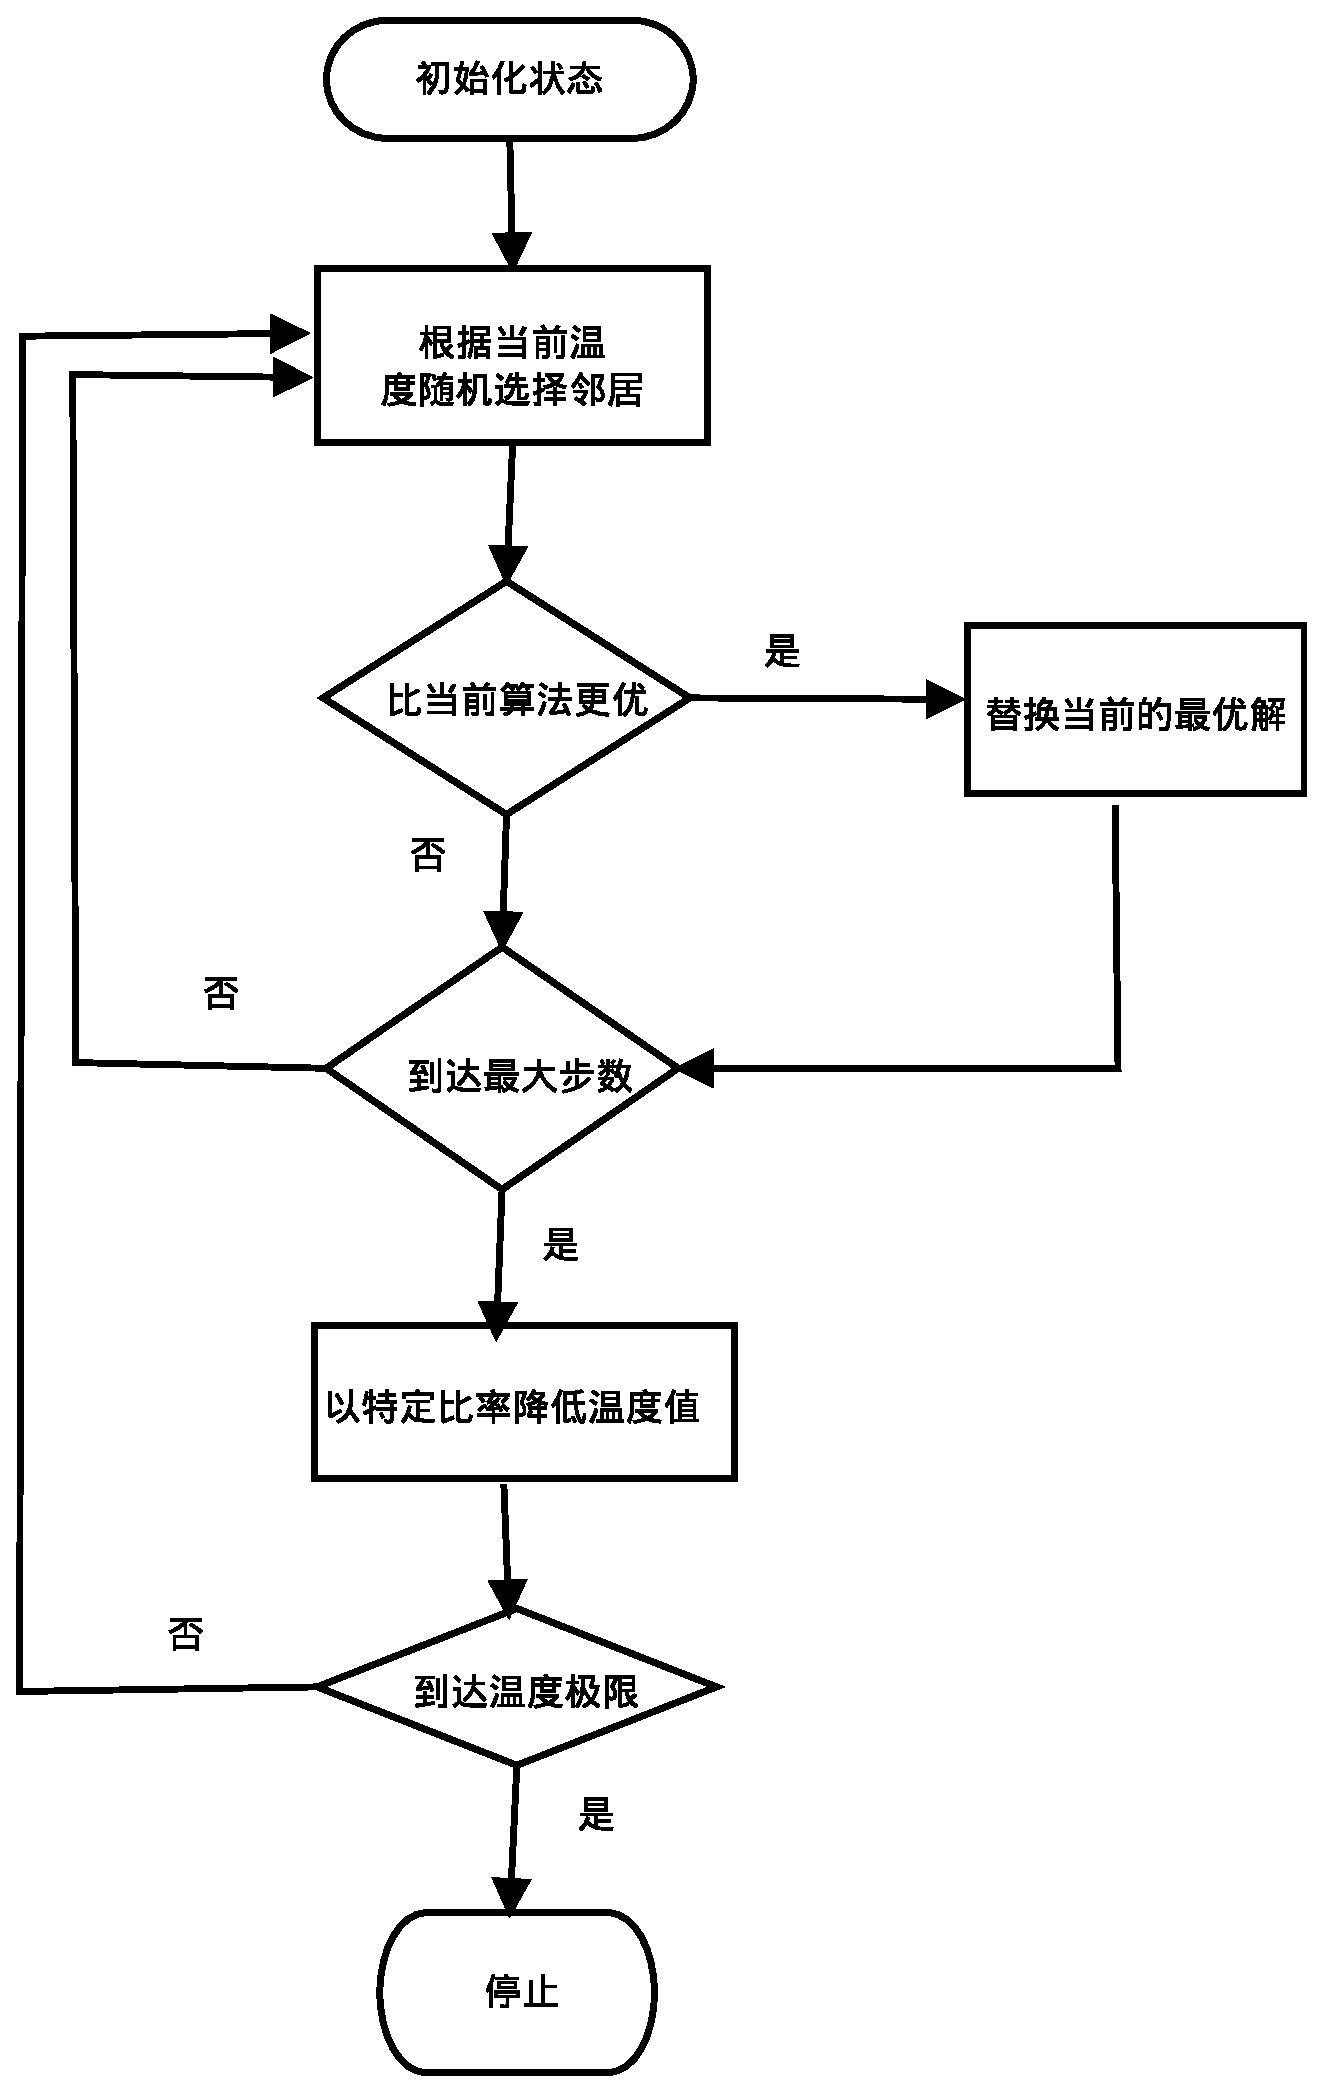
\includegraphics[width=0.6\textwidth]{simulatedannealing}
    \caption{模拟退火算法流程图}\label{fig:simulatedannealing}
    \vspace{\baselineskip}
    \end{figure}

\section{实验结果}
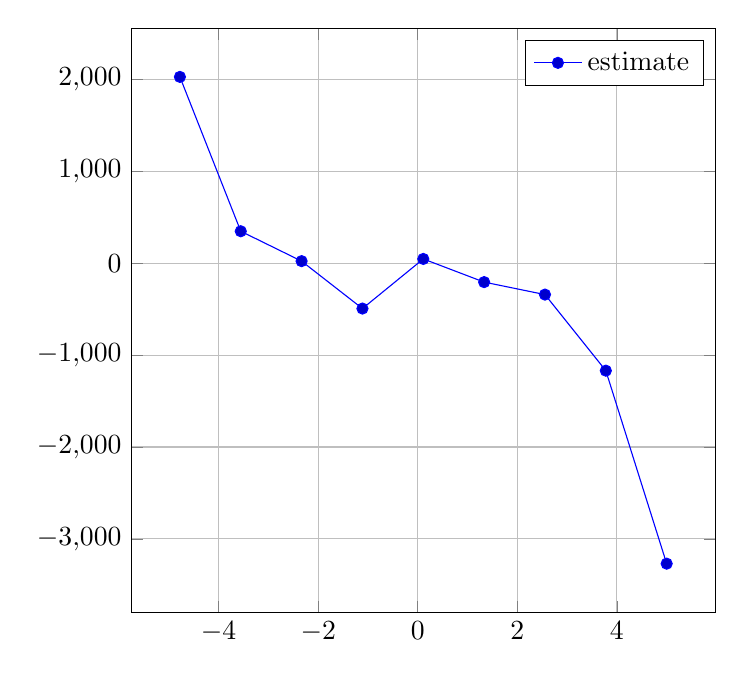
\begin{tikzpicture}
\begin{axis}[
height=9cm,
width=9cm,
grid=major,
]
%\addplot gnuplot[id=filesuffix]{(-x**5 - 242)};
%\addlegendentry{model}
\addplot coordinates {
(-4.77778,2027.60977)
(-3.55556,347.84069)
(-2.33333,22.58953)
(-1.11111,-493.50066)
(0.11111,46.66082)
(1.33333,-205.56286)
(2.55556,-341.40638)
(3.77778,-1169.24780)
(5.00000,-3269.56775)
};
\addlegendentry{estimate}
\end{axis}
\end{tikzpicture}
%http://en.wikipedia.org/wiki/Simulated_annealing
